\documentclass[a4paper]{article}

\usepackage{tecnico_relatorio}

%\usepackage{textcomp}
\usepackage[hypcap]{caption} % makes \ref point to top of figures and tables
%\usepackage{rotating}
\usepackage{float}
%\usepackage[nottoc]{tocbibind}
\usepackage[utf8]{inputenc}
\usepackage{graphicx}
%\usepackage[justification=centering]{caption}
%\usepackage{listings}
\usepackage{indentfirst} % indent first paragraph in section
\usepackage{geometry}	% margins

\begin{document}

	\trSetImage{img/tecnico_logo}{6cm} % Logotipo do Técnico
	\trSetCourse{Mestrado em Engenharia Electrotécnica \\e de Computadores}
	\trSetSubject{Programação de Sistemas}
	%\trSetType{2ª Parte}
	\trSetTitle{Projecto}
	\trSetBoxStyle{0.3}
	\trSetGroupNo{Grupo 3}
	\trSetAuthorNr{2}
	\trSetAuthors
	{
		\begin{center}
			Gonçalo Ribeiro

			73294
		\end{center}
	}{
		\begin{center}
			Miraje Gentilal

			73547
		\end{center}
	}

	\trSetProfessor{Prof. João Nuno de Oliveira e Silva}
	\trMakeCover

	\tableofcontents
	\pagenumbering{gobble}

	\pagebreak

	\pagenumbering{arabic}
	\setcounter{page}{1}


	\section{Arquitetura do Servidor}

	Através da \autoref{fig:architecture} pode-se verificar que a arquitetura é constituída por: 

	\begin{itemize}
		\item Server-Controller : Que vai corresponder ao programa no qual se introduz os comandos a executar no servidor; 
		\item Servidor : Que representa o próprio servidor; 
		\item Relauncher : Permite relançar o servidor em caso de ocorrer um ``crash"; 
		\item Cliente : Representa cada cliente que se liga ao servidor; 
		\item FIFOS : Utilizadas para a comunicação; 
		\item Threads : Utilizadas para processar dados em simultâneo; 
		\item Ligações TCP : Para realizar a comunicação do servidor com os clientes utilizando o protocolo estipulado. 
	\end{itemize}

	\begin{figure}[h]
		\centering
		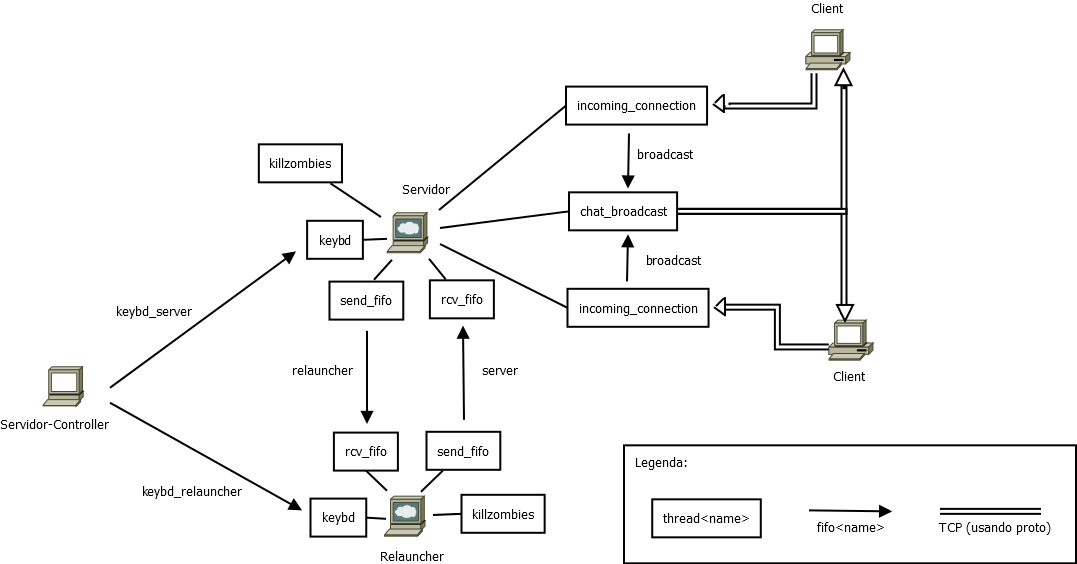
\includegraphics[width=\textwidth]{img/architecture}
		\caption{Diagrama de blocos representativo da arquitetura.}
		\label{fig:architecture}
	\end{figure}


	\subsection{Implementação das Componentes}

	O servidor foi implementado de forma modular, sendo que é possível remover ou adicionar componentes com relativa facilidade. Seria possível desativar por exemplo o módulo de recuperação de falhas ou o módulo que trata da comunicação com o operador do servidor sem que a operação das restantes componentes fosse afetada.

	Em vários sítios do projecto são usadas camadas de abstração que tornam transparente a utilização dos módulos por parte do utilizador. Por exemplo, existe um tipo de dados abstrato para lista (\texttt{list.c}) sobre o qual se constrói a lista de clientes (\texttt{clientlist.c}), sendo que as operações oferecidas ao utilizador nesta última lista são apenas adição e remoção. O programador não tem acesso à estrutura interna dos dados. Sabe apenas que pode guardar e recuperar informação.

	Para o módulo de armazenamento de mensagens usou-se a mesma abordagem: o módulo oferece um interface ao utilizador, que esse utiliza sem saber os pormenores da implementação. Seria possível alterar completamente a implementação do módulo desde que a interface permanecesse igual.

	Outro exemplo de abstração é o módulo \texttt{protobufutils.c}. Este módulo escreve \textit{protocol buffers} para \textit{file descriptors}, o que pode ser usado para enviar \textit{buffers} via TCP, FIFOs, etc. Adicionalmente, este módulo implementa transmissão com \textit{length-prefix framing} (ver \autoref{subsec:length-prefixe_framing}), que é transparente para o utilizador.

	O servidor utiliza nó máximo dois processos em cada momento (um para o servidor em si e outra para o \textit{relauncher})  e um número de \textit{threads} que cresce linearmente com o número de clientes que estão ligados ao servidor. O cliente é constituído apenas por uma \textit{thread}, sendo que a multiplexagem teclado/TCP é conseguida através da função \texttt{select()}. O controlador do servidor é também constituído por uma única \textit{thread}. Para o cliente podia ter sido adotada uma solução com duas \textit{threads}, mas isto não foi feito porque o cliente não ser o ponto central do projecto e porque o \texttt{select()} chegava para resolver a multiplexagem.


	\subsection{Comunicação entre Componentes}

	A comunicação implementada baseia-se no protocolo TCP, FIFOs (\textit{named pipes}) e \textit{mutexes}. A interação com o cliente é feita via TCP e a interação entre as componentes do servidor é feita via FIFOs (ver \autoref{fig:architecture}). É de notar que seria fácil alterar a implementação para que fosse utilizado TCP noutras componentes de comunicação, por exemplo com o objectivo de o servidor poder ser operado remotamente. 

	Por cada cliente existe uma \textit{thread} que recebe e processa os pedidos dos clientes. Quando o pedido é um CHAT a mensagem é transmitida para \textit{thread} de \textit{broadcast}, que difunde a mensagem por todos os clientes ligados ao servidor. Seria possível ter várias \textit{threads} de \textit{broadcast} e repartir os clientes entre elas para aliviar o trabalho de cada uma se o número de clientes crescesse muito.



	\section{Paralelismo}

	O paralelismo é obtido através do uso de processos e de \textit{threads}. De início recorre-se à função \texttt{fork()} para se criar um processo onde se irá executar o servidor. Isto é realizado no \texttt{main()} ficando assim este a executar o \textit{relauncher} e o ``filho" resultante do \texttt{fork()} a executar o servidor, garantido assim que ambos estão a ser executados simultaneamente . 

	O servidor tem se 5 \textit{threads} de base a que se acrescenta uma sempre que é adicionado um cliente, assim tem-se:

	\begin{itemize}
		\item \texttt{thread\_send\_fifo} : É utilizada para enviar \textit{heartbeats} para uma FIFO de forma a comunicar com o \textit{relauncher} informando-o de que está vivo e não há necessidade de relançar o servidor; 
		\item \texttt{thread\_rcv\_fifo} : Funciona de forma oposta à anterior, pois aqui recebe \textit{heartbeats} para uma FIFO que são enviados pelo \textit{relauncher} de forma a indicar o servidor do estado do mesmo; 
		\item \texttt{thread\_killzombies} : Como o nome indica, é utilizada apenas para garantir que em caso de existir um ``crash" e após relançar o servidor não restam processos defuntos. 
		\item \texttt{thread\_keybd} : É utilizada tendo em vista a comunicação com outro programa que irá servir para transmitir para o servidor os comandos de LOG e QUIT, esta comunicação é feita através de FIFOS também, no entanto neste caso apenas existem uma onde o programa de controlo escreve e o servidor lê. 
		\item \texttt{thread\_chat\_broadcast} : É a \textit{thread} que é utilizada para enviar uma mensagem recebida para todos os clientes que estão conectados ao servidor; 
		\item \texttt{thread\_incoming\_connection} : É uma \textit{thread} que é criada cada vez se conecta um novo cliente e é responsável pela comunicação com o mesmo. 
	\end{itemize}

	Como se pode verificar pelas \textit{threads} utilizadas o paralelismo é garantido pois a escrita e receção dos \textit{heartbeats} pode ser feita em simultâneo, bem como a receção de uma mensagem e o seu envio para todos os clientes conectados 
	O \textit{relauncher} tem se 4 \textit{threads}: 

	\begin{itemize}
		\item \texttt{thread\_send\_fifo}, 
		\item \texttt{thread\_rcv\_fifo}; 
		\item \texttt{thread\_killzombies}; 
		\item \texttt{thread\_keybd}. 
	\end{itemize}

	Não se apresenta nenhuma descrição pois têm a mesma funcionalidade que as \textit{threads} associadas ao servidor. Contudo, é de notar que a \texttt{thread\_keybd} aqui apenas serve para verificar a introdução do comando QUIT por parte do utilizador.

	Uma preocupação que foi tida em conta pelo grupo na construção da estrutura do projeto foi o facto de ser possível correr vários servidores em simultâneo. Para tal, utilizou-se o PID do processo que é corrido primeiro (o da função \texttt{main()}) juntamente com nomes predefinidos para criar todas as FIFOS de modo a garantir que não existe conflitos entre FIFOS associados a servidores distintos.




	\section{Estruturas de Dados do Servidor}

	As funcionalidades do servidor requerem a utilização de diversas estruturas de dados. As principais estruturas são: 

	\begin{itemize}
		\item chat storage (\texttt{chatstorage.c}) 
		\item lista de clientes (\texttt{clientlist.c}) 
		\item log (\texttt{logging.c}). 
	\end{itemize}

	De seguida descrevem-se estas estruturas bem como os problemas decorrentes de várias \textit{threads} lhes acederem.
	
	\subsection{Chat Storage}

	\begin{verbatim}
struct chatdb { 
    char **messages; 
    unsigned nr_messages;   // the next free index in `messages' 
    unsigned max_messages;  // the length of chatdb.`messages' array 
};
	\end{verbatim}
	
	Esta estrutura de dados guarda as mensagens dos utilizadores. Devido aos QUERY's pretende-se um acesso rápido a secções da base de dados. Para além disso não é requerido que sejam removidas mensagens. Por estes motivos a estrutura escolhida baseia-se num vector dinâmico de apontadores para mensagens. No início do programa são alocados \texttt{CS\_STEP} (1024) ponteiros para strings. Cada vez que chega uma mensagem é alocada memória à conta para esta string (ou seja são suportadas strings arbitrariamente longas, sem desperdiçar memória) e o ponteiro para esta string é colocado na próxima posição livre de \texttt{messages}. Quando se tenta adicionar uma nova mensagem e o vector de ponteiros se encontra totalmente preenchido o vector é realocado, sendo o seu tamanho aumentado em \texttt{CS\_STEP}.
	
	Este módulo é totalmente transparente para o utilizador. A sua implementação pode ser completamente reformulada desde que se mantenha a interface com o utilizador, que é constituída basicamente por uma função que adiciona uma mensagem e outra que permite recuperar as mensagens entre dois índices. Existem também funções que permitem construir uma nova base de dados e destruir uma existente.

	\subsection{Lista de Clientes} 
	
	A lista de clientes é implementada como uma lista ligada, em que o conteúdo de cada nó é a seguinte estrutura: 
	
	\begin{verbatim}
typedef struct clientinfo { 
    int fd;  
    char *username; 
} clientinfo; 
	\end{verbatim}

 
Os dados guardados são o \textit{username} do cliente e o \textit{file descriptor} associado à sessão TCP com esse cliente. A lista de clientes (\texttt{clientlist.c}) está implementada sobre uma lista que é um tipo abstrato de dados (\texttt{list.c}). É possível a inserção e remoção em qualquer posição da lista. A implementação da lista de clientes também é transparente para o utilizador.

	\subsection{Log} 
 
	O log consiste simplesmente num ficheiro que é criado e aberto em modo \textit{append}. Cada vez que ocorre um evento (start, login, chat, query, disconnect, stop) é adicionada uma nova linha ao log com a informação relativa ao evento. Os eventos relacionados com ações do cliente guardam o \textit{username} do cliente que despoletou o evento. O conteúdo dos chats não é guardado visto que se considerou que não seria relevante para o log. 

	De forma a poder ter vários servidores a correr ao mesmo tempo com logs independentes o ficheiro de log inclui o número do processo inicial do programa. Desta forma desde que o programa é iniciado até ao seu termino todos os eventos relativos a essa sessão são guardados no mesmo ficheiro. Da próxima vez que o servidor for lançado ou se se lançarem dois servidores em paralelo os logs dos dois são distintos. No entanto, no caso de o servidor ``crashar" o novo processo do servidor continua a usar o mesmo log. 

	\subsection{\textit{Race Conditions}}

	A maioria do projeto é baseado na utilização de \textit{threads}, logo é necessário garantir que estas funcionam de forma adequada e com os valores e parâmetros corretos. Sendo assim, o acesso a cada uma das variáveis/estruturas que é partilhada pelas \textit{threads} torna-se numa região critica levando à condição de que esta apenas é modifica e/ou lida por uma e uma só \textit{thread} de cada vez. Para cumprir estes requisitos utiliza-se \textit{mutexes} num total de três, mais especificamente: 

	\begin{itemize}
		\item \texttt{mutex\_clist} : Este \textit{mutex} é utilizado sempre que se acede a uma função relacionada com a lista de clientes (estas funções iniciam o nome com \texttt{CL}) pois é necessário garantir que todas as \textit{threads} acedem à mesma versão da lista de clientes e sem discrepâncias, tornando-se assim uma forma de sincronizar a lista de clientes;  
		\item \texttt{mutex\_log} : Como existe uma \textit{thread} dedicada a cada cliente, várias \textit{threads} podem registar no log mensagens relativas a esses clientes (como mensagens de login, queries, etc.). Caso mais que uma \textit{thread} aceda ao log simultaneamente o acesso e a escrita ao ficheiro de log pode tornar o mesmo corrompido. Assim utiliza-se este \textit{mutex} sempre que se acede e se escreve no log para evitar tais situações. 
		\item \texttt{mutex\_chatdb} : No caso da lista de mensagens existe o problema de que vários clientes podem fazer QUERY's ao mesmo tempo que outros fazem CHAT. É preciso tomar o cuidado de que apenas uma \textit{thread} de cada vez pode adicionar uma mensagem e de que enquanto uma está a adicionar uma nova mensagem não pode haver outra a fazer QUERY's das mensagens. Assim, utiliza-se este \textit{mutex} para garantir o acesso de apenas uma \textit{thread}, de modo a evitar comportamentos indesejados.
	\end{itemize}




	\section{Tolerância a Falhas}

	Sendo este um projeto de ``Programação de Sistemas" é necessário ter um mínimo de garantias para se ter um correto funcionamento perante situações anómalas como comportamento indesejado por parte do utilizador, falhas de comunicação, falhas do sistema, entre outras.  

	Deste modo, o grupo implementou um dos mecanismos lecionados nas aulas teóricas e laboratoriais para o caso de o servidor ``crashar": a utilização de um \textit{relauncher} que comunica com o servidor através \textit{heartbeats} que são enviadas em FIFOS (tendo, portanto o servidor e o \textit{relauncher} uma FIFO destinada apenas para a receção e outra apenas para o envio). Caso passe um determinado tempo e não seja recebido um \textit{heartbeat} (tanto por parte do servidor como do \textit{relauncher}) o que não o enviou é relançado pelo outro. 

	Esta solução gera um inconveniente, como um processo relança outro é perdida a ``ligação" com o terminal associado ao programa inicial pois o processo que era ``pai" (e tinha o terminal associado) pode-se tornar ``filho" (que sendo um processo diferente deixa de estar associado ao terminal). Consequentemente, caso o processo original morra deixa-se de poder enviar os comandos LOG e QUIT que controlam o servidor. Para contornar esta situação recorre-se a um outro programa que se chamou de \texttt{server-controller} que serve como ponte de comunicação entre o operador e o servidor, permitindo a execução dos comandos anteriormente referidos. Os comandos são introduzidos no \texttt{server-controller} e transferidos para o servidor, que age de acordo com os mesmos e imprime os resultados no ecrã. Esta solução foi alcançada recorrendo novamente a FIFOS, criando um FIFO para comunicação com o servidor e outra para comunicação com o \textit{realuncher}. A FIFO para o \textit{relauncher} é necessária porque queremos que ambos os processos terminem em simultâneo, de forma a evitar que o \textit{relauncher} volte a lançar o servidor. Podia ter sido usada a própria FIFO do \textit{crash recovery} para o servidor informar o relauncher de que também devia terminar, mas isto não foi feito para que o módulo \texttt{crashrecovery.c} seja independente do módulo que recebe comandos do operador. Os resultados dos comandos podiam ter sido transferidos de volta para o \texttt{controller} e ser esse programa a mostra-los, mas considerou-se que não se ganharia muito em fazer isso para este projecto, pelo que os resultados dos comandos LOG e QUIT são mostrados no terminal em que o servidor foi lançado. Bastaria criar uma FIFO com o sentido servidor/controlador, através da qual seria transmitido um \textit{protocol buffer} com os resultados gerados pelo servidor, que seriam depois impressos no ecrã do controlador.

	Para o caso de falhas de comunicação e de sistema garantiu-se que é apresentada uma mensagem adequada ao utilizador e termina-se o programa corretamente, com um código de erro.




	\section{Comunicação}

	Existem vários canais de comunicação neste projecto: 

	\begin{itemize}
		\item ligação TCP entre cliente e servidor 
		\item FIFOs entre \textit{server} e \textit{relauncher} 
		\item FIFO para a \textit{thread} de \textit{broadcast} 
		\item FIFOs para para controlar o servidor e o \textit{relauncher} através de um processo externo. 
	\end{itemize}

	Em geral foram usados \textit{protocol buffers} como forma de empacotar as mensagens que são transmitidas. Tal como visto nas aulas este sistema tem várias vantagens face a outras formas de comunicação, como mensagens mais compactas e que respeitam a \textit{endianness} das máquinas envolvidas na comunicação.

	\subsection{\textit{Length-Prefix Framing}}
	\label{subsec:length-prefixe_framing}

	A utilização de \textit{protocol buffers} com campos \texttt{str} e \texttt{repeated} traz um problema: não sabemos à partida qual o tamanho das mensagens que estão a ser transferidas. A implementação de \textit{protocol buffers} utilizada no projecto não dispõe de uma forma de delimitar várias mensagens consecutivas que estejam no mesmo canal (\textit{framing}).

	De forma a mitigar este problema decidiu implementar-se \textit{length-prefix framing}. Este é um método de delimitação de mensagens (ou \textit{frames}) que consiste em transmitir a mensagem real precedida do seu tamanho. Nesta caso implementou-se um prefixo de 4 bytes, o que permitiria o funcionamento correto até mensagens de 4 GiB. Quando uma mensagem é recebido o recetor pode verificar qual o tamanho do \textit{buffer} que deve alocar de forma a ter espaço para receber a totalidade da mensagem. Sabe também onde começa a próxima mensagem.

	Para não arruinar um dos objetivos dos \textit{protocol buffers} foi tido o cuidado de respeitar a \textit{endianness} das máquinas envolvidas na comunicação, fazendo uso das funções \texttt{htonl()} e \texttt{ntohl()}---que ``conhecem" a \textit{endianess} das máquinas em que estão a correr---para que as máquinas envolvidas interpretassem corretamente o prefixo.

	É óbvio que usar este método de \textit{framing} traz problemas de segurança visto que um atacante pode fazer o servidor alocar quantidades grandes (neste caso 4 GB) de memória, esgotando os recursos do servidor. No entanto, este problema não faz parte do âmbito desta cadeira nem dos problemas centrais do projecto, pelo que não foi mitigado.

	\subsection{Cliente/Servidor}

	As mensagens envolvidas na comunicação TCP têm a seguinte descrição:

	\begin{verbatim}
message ClientToServer 
{ 
    enum Type { 
        LOGIN = 0; 
        DISC = 1; 
        CHAT = 2; 
        QUERY = 3; 
    } 
 
    required Type type = 1; // identify type of message 
    optional string str = 2;    // used for LOGIN (username) and CHAT (string) 
    optional uint64 id_min = 3; // used for QUERY 
    optional uint64 id_max = 4; 
}
	\end{verbatim}

	\begin{verbatim}
message ServerToClient 
{ 
    enum Code { 
        OK = 0; 
        NOK = 1; 
    } 
 
    optional Code code = 1; // used for LOGIN only 
    repeated string str = 2;    // used for QUERY and to receive chats 
}
	\end{verbatim}

	Como se pode verificar, existe uma mensagem do cliente para o servidor e outra do servidor para o cliente. Na mensagem do cliente para o servidor existe um tipo enumerado que identifica o tipo do pedido que é feito ao servidor. Do lado do servidor existe uma máquina de estados que verifica os tipos dos pedidos e age de acordo com o tipo de novos pedidos face a pedidos passados. O campo \texttt{str} é usado em dois dos tipos de mensagem: nas mensagens de LOGIN é usado para transferir o \textit{username}; e nas mensagens de CHAT transfere o chat que o utilizador pretende enviar. Os dois campos de inteiros são usados para as QUERY's, em que é necessário transmitir um índice mínimo e máximo das mensagens que se pretende consultar. 

	As mensagens do servidor têm um campo enumerado que é usado para informar o cliente se o LOGIN foi feito com sucesso (ou seja se não existia alguém com o \textit{username} com que foi feito login) ou se falhou. Existe ainda um campo repetido para strings, que tem duas funções: no caso de respostas a QUERY's este campo contém a série de mensagens correspondentes à query (ou nenhuma caso não haja mensagens correspondentes ao índices pedidos); e no caso de receção de um chat este campo contém a mensagem enviada por outro cliente. 

	\subsection{Servidor/Relauncher}  

	As mensagens transferidas entre o servidor e o \textit{relauncher} não têm conteúdo definido. Ambos os processos precisam apenas de garantir que o outro está vivo do outro lado da FIFO. Para isto basta enviar periodicamente um byte para a FIFO, não interessando qual o valor desse byte. 

	\subsection{Broadcast} 

	\begin{verbatim}
message ServerToBroadcast 
{ 
    required string str = 1;    // the message (chat) sent by the client 
}
	\end{verbatim} 

	Os chats dos clientes são recebidos por \textit{threads} do servidor. A cada cliente está associada uma \textit{thread}. Quando uma destas \textit{threads} recebe um novo chat este tem que ser transmitido para todos os clientes. A solução adotada é ter uma \textit{thread} que recebe os chats numa FIFO e que os envia para todos os clientes que estão na lista de clientes. A mensagem definida para esta comunicação contém um único campo, em que é colocada a mensagem a enviar. Da mensagem faz parte o nome do cliente que a enviou, que é colocado antes da mensagem propriamente dita. 

	\subsection{Controlador/Servidor}

	\begin{verbatim}
message ControllerToServer 
{ 
    enum Type { 
        LOG = 0; 
        QUIT = 1; 
    } 
 
    required Type type = 1; // identify type of command 
}
	\end{verbatim}

	De forma a poder controlar o servidor (e o \textit{relauncher}) chama-se um programa à parte (o controlador). Este programa envia dois tipos de mensagens ao servidor (e ao \textit{relauncher}): uma mensagem de LOG ou uma de QUIT. Sendo assim o \textit{protocol buffer} definido contém um único campo, enumerado, que transmite o código correspondente à ação que o servidor deve tomar. 


	\section{Testes de Unidades}

	Para testar o módulo de chat realizou-se um conjunto de 6 testes, os quais pretendiam verificar o correto funcionamento de todas as vertentes do módulo, assim para cada um dos testes no inicio cria-se uma estrutura \texttt{chatdb} (em \texttt{setUp()} recorrendo à função \texttt{CSinit()}) e no final elimina-se a mesma (em \texttt{tearDown()} recorrendo à função \texttt{CSdestroy()}). Segues-se uma breve descrição para cada um dos testes.

	\begin{enumerate}
		\item \texttt{test\_db\_creation()} : Este teste é utilizado para confirmar se a inicialização da base de dados foi feita corretamente, para tal, verifica-se se primeiramente se foi alocado espaço para a estrutura (assim o ponteiro para a \texttt{chatdb} não pode ser \texttt{NULL}) e de seguida confirma-se o tamanho desta (que tem de ser 0). 
		\item \texttt{test\_add\_message()} : Este simples teste verifica se após a adição de uma mensagem (utilizando a função \texttt{CSstore()}) o número de mensagens presentes na base de dados aumentou em uma unidade. 
		\item \texttt{test\_single\_query()} : Após adicionar uma mensagem é necessário verificar se a mensagem adicionada está correta, bem como se a função que permite realizar os QUERY's funciona corretamente. Assim através da função \texttt{CSquery()} pede-se apenas uma mensagem e verifica-se se corresponde à mensagem que foi adicionada. 
		\item \texttt{test\_limit()} : Como a estrutura está definida para alocar um máximo inicial de 1024 mensagens (por definição do parâmetro \texttt{CS\_STEP}) é necessário garantir que mesmo após a passagem deste limite continua-se a guardar as mensagens. Este teste serve para isso mesmo, cria 1500 mensagens e guarda-as na estrutura, após o que verifica se o número de mensagens guardadas é de facto 1500. 
		\item \texttt{test\_multiple\_query()} : Após testar a capacidade da base de dados e de verificar que uma \texttt{query} de uma mensagem é feita com sucesso, é necessário testar uma \texttt{query} de várias mensagens. Assim, cria-se 1500 mensagens distintas e guarda-se cada uma delas, depois realiza-se uma \texttt{query} para mensagens do índice 750 até ao índice 1250 e confirma-se se cada uma delas corresponde ao que foi guardado para o respetivo índice. Estes índices foram escolhidos porque permitem testar que as mensagens continuam a ser corretamente guardadas mesmo depois de ter havido uma expansão da base de dados (quando se ultrapassam as 1024 (\texttt{CS\_STEP}) mensagens).
		\item \texttt{test\_change\_length\_db()} : Num dos testes anteriores confirma-se se é possível exceder a capacidade inicial de mensagens definida para a base de dados, no entanto, é necessário verificar se o novo limite é feito corretamente, ou seja, verifica-se se o \texttt{realloc()} foi feito com o novo limite definido pelo utilizador (que foi feito de forma a incrementar \texttt{CS\_STEP} posições cada vez que se atinge o limite de mensagens).
	\end{enumerate}


	\section{Compilação e Utilização dos Programas}

	Em conjunto com o código (pasta \texttt{src}) é fornecido um \texttt{makefile} que permite a compilação dos três programas. Basta correr o comando \texttt{make} para que os 3 sejam compilados. Os programas resultantes serão 

	\begin{enumerate}
		\item \texttt{client} 
		\item \texttt{server} 
		\item \texttt{server-controller} 
	\end{enumerate}

	O servidor aceita um argumento opcional que permite escolher a porta em que o servidor deve ser corrido. Exemplo:

	\begin{verbatim}
	./server -p 3001 
	\end{verbatim}

	O cliente aceita dois argumentos opcionais: um para escolher o endereço IP do servidor e outro para escolher a porta em que o servidor está à escuta. Exemplo:

	\begin{verbatim}
	./client -i 127.0.0.1 -p 3001
	\end{verbatim}

	O controlador requer um parâmetro obrigatório, que é o PID original do servidor que se quer controlar. Quando o servidor é lançado o seu PID é impresso e é esse PID que deve ser usado. É também possível ver os PIDs dos servidores que estão a correr correndo o comando \texttt{ls /tmp/server-*}. Exemplo: 

	\begin{verbatim}
	./server-controller 4321 
	\end{verbatim}

	Os testes do módulo \texttt{chatstorage.c} encontram-se na pasta \texttt{testing}. Nesta pasta encontra-se também um \texttt{makefile} que automatiza a criação do projecto necessário para correr os testes. O \texttt{makefile} da pasta \texttt{src} também pode ser usado para correr os testes, fazendo \texttt{make tests}.


	\section{Conclusões e Comentários}

	Durante o desenvolvimento do projeto foi-se percebendo a importância dos mecanismos de sincronização, da utilização de protocolos de comunicação e a utilidade dos diferentes meios de comunicação entre processos, especialmente das FIFO's que foi o que foi mais utilizado, juntamente com os mecanismos de paralelização, que é essencial na programação de qualquer sistema de complexidade moderada. Compreendeu-se também que é necessário recorrer a \textit{mutexes} de forma a garantir consistência nos dados e o correto funcionamento do programa. Por fim, aprendeu-se a construir testes específicos para módulos do programa, neste caso apenas para o módulo de armazenamento das mensagens, e o quão útil estes podem ser para descobrir eventuais erros de programação e problemas da implementação. 

	De uma forma geral, o projeto contribui para consolidar a matéria lecionada nas aulas teóricas e laboratoriais.

\end{document}
